% Options for packages loaded elsewhere
\PassOptionsToPackage{unicode}{hyperref}
\PassOptionsToPackage{hyphens}{url}
\documentclass[
  11pt,
]{article}
\usepackage{xcolor}
\usepackage[margin=1in, includeheadfoot]{geometry}
\usepackage{amsmath,amssymb}
\setcounter{secnumdepth}{5}
\usepackage{iftex}
\ifPDFTeX
  \usepackage[T1]{fontenc}
  \usepackage[utf8]{inputenc}
  \usepackage{textcomp} % provide euro and other symbols
\else % if luatex or xetex
  \usepackage{unicode-math} % this also loads fontspec
  \defaultfontfeatures{Scale=MatchLowercase}
  \defaultfontfeatures[\rmfamily]{Ligatures=TeX,Scale=1}
\fi
\usepackage{lmodern}
\ifPDFTeX\else
  % xetex/luatex font selection
\fi
% Use upquote if available, for straight quotes in verbatim environments
\IfFileExists{upquote.sty}{\usepackage{upquote}}{}
\IfFileExists{microtype.sty}{% use microtype if available
  \usepackage[]{microtype}
  \UseMicrotypeSet[protrusion]{basicmath} % disable protrusion for tt fonts
}{}
\usepackage{setspace}
\makeatletter
\@ifundefined{KOMAClassName}{% if non-KOMA class
  \IfFileExists{parskip.sty}{%
    \usepackage{parskip}
  }{% else
    \setlength{\parindent}{0pt}
    \setlength{\parskip}{6pt plus 2pt minus 1pt}}
}{% if KOMA class
  \KOMAoptions{parskip=half}}
\makeatother
\usepackage{graphicx}
\makeatletter
\newsavebox\pandoc@box
\newcommand*\pandocbounded[1]{% scales image to fit in text height/width
  \sbox\pandoc@box{#1}%
  \Gscale@div\@tempa{\textheight}{\dimexpr\ht\pandoc@box+\dp\pandoc@box\relax}%
  \Gscale@div\@tempb{\linewidth}{\wd\pandoc@box}%
  \ifdim\@tempb\p@<\@tempa\p@\let\@tempa\@tempb\fi% select the smaller of both
  \ifdim\@tempa\p@<\p@\scalebox{\@tempa}{\usebox\pandoc@box}%
  \else\usebox{\pandoc@box}%
  \fi%
}
% Set default figure placement to htbp
\def\fps@figure{htbp}
\makeatother
% definitions for citeproc citations
\NewDocumentCommand\citeproctext{}{}
\NewDocumentCommand\citeproc{mm}{%
  \begingroup\def\citeproctext{#2}\cite{#1}\endgroup}
\makeatletter
 % allow citations to break across lines
 \let\@cite@ofmt\@firstofone
 % avoid brackets around text for \cite:
 \def\@biblabel#1{}
 \def\@cite#1#2{{#1\if@tempswa , #2\fi}}
\makeatother
\newlength{\cslhangindent}
\setlength{\cslhangindent}{1.5em}
\newlength{\csllabelwidth}
\setlength{\csllabelwidth}{3em}
\newenvironment{CSLReferences}[2] % #1 hanging-indent, #2 entry-spacing
 {\begin{list}{}{%
  \setlength{\itemindent}{0pt}
  \setlength{\leftmargin}{0pt}
  \setlength{\parsep}{0pt}
  % turn on hanging indent if param 1 is 1
  \ifodd #1
   \setlength{\leftmargin}{\cslhangindent}
   \setlength{\itemindent}{-1\cslhangindent}
  \fi
  % set entry spacing
  \setlength{\itemsep}{#2\baselineskip}}}
 {\end{list}}
\usepackage{calc}
\newcommand{\CSLBlock}[1]{\hfill\break\parbox[t]{\linewidth}{\strut\ignorespaces#1\strut}}
\newcommand{\CSLLeftMargin}[1]{\parbox[t]{\csllabelwidth}{\strut#1\strut}}
\newcommand{\CSLRightInline}[1]{\parbox[t]{\linewidth - \csllabelwidth}{\strut#1\strut}}
\newcommand{\CSLIndent}[1]{\hspace{\cslhangindent}#1}
\setlength{\emergencystretch}{3em} % prevent overfull lines
\providecommand{\tightlist}{%
  \setlength{\itemsep}{0pt}\setlength{\parskip}{0pt}}
\usepackage[dvipsnames]{xcolor}
\definecolor{TitleBlue}{HTML}{0E2A47}
\definecolor{AccentBlue}{HTML}{1F6F8B}
\definecolor{RuleGray}{HTML}{C9D6E3}
\usepackage{float}
\usepackage{booktabs}
\usepackage{longtable}
\usepackage{array}
\usepackage{multirow}
\usepackage{threeparttable}
\usepackage{amsmath}
\usepackage{amssymb}
\usepackage{graphicx}
\usepackage{setspace}
\usepackage{caption}
\captionsetup{font=small, labelfont={bf,color=TitleBlue}, justification=raggedright, singlelinecheck=false}
\renewcommand{\arraystretch}{1.12}
\setlength{\tabcolsep}{6pt}
\setlength{\LTleft}{0pt}
\setlength{\LTright}{0pt}
\setlength{\belowcaptionskip}{6pt}
\setlength{\abovecaptionskip}{4pt}
\setlength{\textfloatsep}{12pt plus 2pt minus 2pt}
\setlength{\floatsep}{10pt plus 2pt minus 2pt}
\setlength{\intextsep}{10pt plus 2pt minus 2pt}
\floatplacement{figure}{H}
\floatplacement{table}{H}
\setcounter{tocdepth}{2}
\makeatletter
\renewcommand{\section}{\@startsection{section}{1}{\z@}{-2.0ex \@plus -0.5ex \@minus -.2ex}{0.8ex \@plus.2ex}{\normalfont\Large\bfseries\color{TitleBlue}}}
\renewcommand{\subsection}{\@startsection{subsection}{2}{\z@}{-1.6ex\@plus -0.5ex \@minus -.2ex}{0.6ex \@plus.2ex}{\normalfont\large\bfseries\color{TitleBlue}}}
\renewcommand{\subsubsection}{\@startsection{subsubsection}{3}{\z@}{-1.2ex\@plus -0.5ex \@minus -.2ex}{0.5ex \@plus.2ex}{\normalfont\normalsize\bfseries\color{AccentBlue}}}
\makeatother
\makeatletter
\def\maketitle{
\begin{titlepage}
\thispagestyle{empty}
\centering
\vspace*{2.1cm}
{\LARGE\bfseries\color{TitleBlue}\@title\par}
\vspace{0.55cm}
{\large\color{AccentBlue}A Conditional Pricing Framework Linking Greenium, Climate Exposure, and Macro-Policy Regimes\par}
\vspace{1.4cm}
{\large\textbf{Authors}\par}
\vspace{0.35cm}
{\large Sathvik Gorle, Nan Zhang, Andrew Zhai, and Richard Mei\par}
\vspace{0.20cm}
{\normalsize North Carolina School of Science and Mathematics\\
Duke University\par}
\vspace{1.4cm}
{\normalsize \@date\par}
\vfill
{\color{RuleGray}\rule{0.86\linewidth}{0.8pt}\par}
\end{titlepage}
\setcounter{page}{1}
}
\makeatother

\usepackage{fancyhdr}
\usepackage{ragged2e}
\clubpenalty=10000
\widowpenalty=10000
\pagestyle{fancy}
\fancyhf{}
\fancyhead[L]{\small\itshape Frequency- and State-Dependent Climate Risk Pricing}
\fancyhead[R]{\small \thepage}
\fancyfoot[C]{}
\renewcommand{\headrulewidth}{0.5pt}
\renewcommand{\footrulewidth}{0pt}
\setlength{\headheight}{14pt}
\renewcommand{\abstractname}{\large Abstract}
\setlength{\parindent}{1.15em}
\setlength{\parskip}{0.35em}
\emergencystretch=2em
\tolerance=2000
\AtBeginDocument{\hypersetup{colorlinks=true,linkcolor=TitleBlue,citecolor=AccentBlue,urlcolor=AccentBlue}}
\usepackage{booktabs}
\usepackage{longtable}
\usepackage{array}
\usepackage{multirow}
\usepackage{wrapfig}
\usepackage{float}
\usepackage{colortbl}
\usepackage{pdflscape}
\usepackage{tabu}
\usepackage{threeparttable}
\usepackage{threeparttablex}
\usepackage[normalem]{ulem}
\usepackage{makecell}
\usepackage{xcolor}
\usepackage{bookmark}
\IfFileExists{xurl.sty}{\usepackage{xurl}}{} % add URL line breaks if available
\urlstyle{same}
\hypersetup{
  pdfauthor={Sathvik Gorle, Nan Zhang, Andrew Zhai, Richard Mei},
  hidelinks,
  pdfcreator={LaTeX via pandoc}}

\title{Frequency- and State-Dependent Climate Risk Pricing\\
in U.S. Green Bond Markets\\[0.4em]
\normalfont\large A Conditional Pricing Framework Linking Greenium, Climate Exposure, and Macro-Policy Regimes}
\author{Sathvik Gorle, Nan Zhang, Andrew Zhai, and Richard Mei\\[0.35em]
\normalfont\normalsize North Carolina School of Science and Mathematics / Duke University}
\date{March 2026}

\begin{document}
\maketitle

{
\setcounter{tocdepth}{3}
\tableofcontents
}
\setstretch{1.15}
\begin{abstract}
\noindent Green bonds finance environmentally sustainable projects, yet it remains unclear how their prices move relative to conventional bonds. Older work spots tiny average discounts (``greeniums'') but shows big swings issuer by issuer. We ask whether climate yardsticks reliably line up with those discounts and whether the story changes with calendar frequency or Fed posture. Combining six Bloomberg green bonds with decade-long market dashboards, monthly Actuaries Climate Risk Index readings flatten green-minus-regular corporate gaps while jittery daily links stay statistically muddy. KRBN sensitivities deepen when tightening is underway. Pooling 130 monthly observations, ACRI lines up with narrower green-minus-regular gaps at roughly the five-percent hurdle once Treasury, IG spreads, and fear gauges are included, while EGARCH evidence still attributes most day-to-day jitter to rates and VIX. Narrative earmarking grades rarely deliver reliable outperformance yet keep issuers accountable in text. Lessons concentrate on month-end horizons when macro gauges are spelled out plainly. The six-bond exercise is illustrative yet outlines a playbook others can scale nationally.

\medskip
\noindent \textbf{Keywords:} Green bonds, greenium, climate risk pricing, transition risk, policy uncertainty, carbon ETF (KRBN), regime dependence
\end{abstract}

\section{Introduction}\label{introduction}

Green bonds are fixed-income securities that finance environmentally sustainable projects but retain the same coupons, durations, ratings, and tax treatments as conventional bonds (\citeproc{ref-karpf2018}{Karpf and Mandel 2018}; \citeproc{ref-baker2022}{Baker et al. 2022}). Issuance spans supranational, municipal, and corporate programs, concentrated in utilities, resilience, renewable power, transport, and water infrastructure (\citeproc{ref-liaw2020}{Liaw 2020}). Green labels have grown quickly, though they remain a fractional share of world bond issuance because placement costs remain high and definitions are uneven across jurisdictions (\citeproc{ref-macaskill2021}{MacAskill et al. 2021}).

The central question is whether labeling produces a repeatable pricing concession (what the literature calls the \textbf{greenium}). Pooled U.S.\ matching evidence typically finds small unconditional wedges of 1--7 basis points (\citeproc{ref-baker2022}{Baker et al. 2022}; \citeproc{ref-partridge2020}{Partridge and Medda 2020}; \citeproc{ref-sojoudi2025}{Sojoudi et al. 2025}). Studies focused on shoreline exposure, utility and municipal subsets, stacked hazards, or emission-policy transitions often report larger spread responses (\citeproc{ref-painter2020}{Painter 2020}; \citeproc{ref-li2024}{Li et al. 2024}; \citeproc{ref-smull2023}{Smull et al. 2023}; \citeproc{ref-bolton2023}{Bolton and Kacperczyk 2023}). Index-level portfolios likewise react to uncertainty and asset-market spillovers with modest spreads once the horizon matches the story (\citeproc{ref-pham2022}{Pham and Nguyen 2022}; \citeproc{ref-park2020}{Park et al. 2020}; \citeproc{ref-tiwari2022}{Tiwari et al. 2022}; \citeproc{ref-mari2024}{Mar'i 2024}).

These research threads have developed mostly independently (\citeproc{ref-baker2022}{Baker et al. 2022}; \citeproc{ref-sojoudi2025}{Sojoudi et al. 2025}; \citeproc{ref-liaw2020}{Liaw 2020}; \citeproc{ref-pham2022}{Pham and Nguyen 2022}; \citeproc{ref-painter2020}{Painter 2020}), so headline numbers from one approach rarely carry over cleanly to another. Typical matched pairs remove coupon ladders but seldom include the issuer-by-risk patterns that shoreline or hazard papers emphasize. Narrow physical-risk work studies munis or utilities yet rarely compares adaptation-minded green bonds to conventional cousins with similar profiles. Aggregate uncertainty work leans on ETF or index totals and often omits issuer detail or same-day IG credit spreads. Matching studies blur calm and turbulent years together, whereas event papers zoom into short trading-day windows. For these reasons one should not expect a single large elasticity from any one design to match coefficients from pooled green-minus-conventional regressions (\citeproc{ref-bolton2023}{Bolton and Kacperczyk 2023}).

Against that backdrop, we treat outcomes as hinging on timeframe and circumstance. Institutional reporting tends to drift month-by-month whereas tick files refresh daily (\citeproc{ref-liaw2020}{Liaw 2020}; \citeproc{ref-sojoudi2025}{Sojoudi et al. 2025}). Results also shift alongside Fed tightening, IRA headlines, or jumpy volatility. Ordinary bond channels---Treasury yields, IG spreads, fear gauges---typically absorb shocks first; climate indicators add meaningful color only after those baselines are modeled (\citeproc{ref-bolton2023}{Bolton and Kacperczyk 2023}; \citeproc{ref-pham2022}{Pham and Nguyen 2022}).

\textbf{Contribution.} This paper fills those gaps in three related steps. First, we combine Bloomberg green and conventional index differentials from January~2014 through December~2025 with ACRI composites, Climate Policy Uncertainty readings from \citeproc{ref-gavriilidis2021}{Gavriilidis (2021)}, KraneShares Global Carbon (\texttt{KRBN}) returns, IRA-era markers, tightening windows keyed to Fed hikes, standardized VIX, and other Bloomberg- and Fed-based series. Second, we keep pooled regressions in the spirit of earlier greenium work but add six Bloomberg issuers framed like \citeproc{ref-flammer2021}{Flammer (2021)}, pairing text-based specificity scores with returns versus a benchmark. Third, we lay out findings by month-level tables, eleven annual observations, daily KRBN interactions, six-name bond vignettes, and appendix vector-autoregression plots.

\textbf{Hypothesized mechanisms.} Following \citeproc{ref-flammer2021}{Flammer (2021)}, financing earmarked for shoreline resilience should coincide with tighter valuations when physical indices rise, whereas green bonds stacked on hazard-heavy operating exposures may cheapen whenever insured losses correlate with cash flows. Hypothesis H4 captures this hedge-versus-amplification split. Tests below stay on diversified indices unless otherwise noted.

\textbf{Relative magnitudes.} Unconditional greeniums in the single-digit basis-point range are naturally dwarfed by rating moves that routinely shift spreads 15--25 basis points, munis whose tax advantages can stretch past eighty basis points, and liquidity premiums documented in trades (\citeproc{ref-baker2022}{Baker et al. 2022}; \citeproc{ref-liaw2020}{Liaw 2020}; \citeproc{ref-macaskill2021}{MacAskill et al. 2021}; \citeproc{ref-partridge2020}{Partridge and Medda 2020}). Treasury yields and IG OAS already swallow much of green-minus-conventional swings before climate variables enter (\citeproc{ref-baker2022}{Baker et al. 2022}), which is why plausible climate slopes need Treasury, spread, and volatility controls akin to portfolio reporting (\citeproc{ref-pham2022}{Pham and Nguyen 2022}).

\textbf{Pooling and disclosure.} Pooling calendars mixes calm issuance years with crisis years (\citeproc{ref-sojoudi2025}{Sojoudi et al. 2025}; \citeproc{ref-liaw2020}{Liaw 2020}). Coupon ladders, seasoning, taxes, liquidity segments, and any unconditional ``green discount'' jointly move spreads (\citeproc{ref-macaskill2021}{MacAskill et al. 2021}). Slow-moving climate composites match poorly with day-by-day regressions unless the horizon lines up with how portfolios rebalance (\citeproc{ref-bolton2023}{Bolton and Kacperczyk 2023}; \citeproc{ref-seltzer2022}{{Seltzer et al.} 2022}). Investor lineup shifts when mandates change (\citeproc{ref-liaw2020}{Liaw 2020}), so a single intercept can misstate average pricing. Ordinary pooled regressions averaging everyone into one line smooth over issuer differences, whereas focused climate papers often study hand-picked crises or regions (\citeproc{ref-painter2020}{Painter 2020}; \citeproc{ref-li2024}{Li et al. 2024}). Breaking results out by monthly vs.\ daily horizons, IRA and tightening indicators, IG OAS, and VIX helps separate real climate swings from quirks created by cramming unlike years together (\citeproc{ref-pham2022}{Pham and Nguyen 2022}).

\textbf{Road map of findings.} Market-factor regressions anchor the tables. Six Bloomberg vignettes document disclosure language rather than national representativeness (\citeproc{ref-flammer2021}{Flammer 2021}). Monthly ACRI rejects a zero coefficient at roughly five percent ($p = 0.048$, $N = 130$). Climate-policy uncertainty shows up cleanly only once months are summed to eleven yearly rows ($N = 11$), a slice too short for textbook large-sample shortcuts. KRBN samples spanning August~2020--December~2024 contain $N = 1{,}614$ trading days after non-missing histories align. Tightening interactions clear the 5\% bar in the simpler KRBN regression (Table~\ref{tab:krbn-main}), whereas adding IRA markers and fuller volatility controls nudges one interaction toward $p \approx 0.064$, partly offset by a post-IRA term near $p \approx 0.049$. Appendix tables list NLP specificity scores, utilities crossed with Climate Policy Uncertainty, and issuance windows tied to each bond's first clean Bloomberg quotes ($p < 0.001$ in Appendix Table~\ref{tab:app-did-6bond} with Figure~\ref{fig:post-issuance-drift-plot}), echoing themes in \citeproc{ref-flammer2021}{Flammer (2021)}. Daily variance splits still show Treasury and IG news driving most of the action. Throughout, slopes describe conditional correlations---the data lack an external instrument needed to pin down causality cleanly.

Section~\ref{literature-and-hypotheses} restates hypotheses against prior evidence. Section~\ref{data-and-empirical-design} documents variable construction. Section~\ref{results} presents estimates. Section~\ref{discussion-and-limitations} spells out limitations. Section~\ref{conclusion} synthesizes implications.

\section{Literature and Hypotheses}\label{literature-and-hypotheses}

\subsection{Green bond pricing and the greenium}

The greenium literature asks whether investors will accept lower yields on green bonds compared to otherwise identical conventional bonds. Several mechanisms could explain a greenium: ESG-oriented investors may be willing to give up yield for environmental outcomes (\citeproc{ref-liaw2020}{Liaw 2020}; \citeproc{ref-baker2022}{Baker et al. 2022}), institutional mandates may compress yields when green supply is limited and demand is high (\citeproc{ref-macaskill2021}{MacAskill et al. 2021}), issuers may use green bonds to signal better environmental management (\citeproc{ref-flammer2021}{Flammer 2021}), and weak verification could produce a greenwashing premium (\citeproc{ref-macaskill2021}{MacAskill et al. 2021}).

Empirically, the U.S.\ municipal market is distinct because federal and state tax breaks already compress yields, leaving little room for additional green rate compression (\citeproc{ref-partridge2020}{Partridge and Medda 2020}). Studies that match on rating, maturity, sector, and tax status find residual green premiums of 2 to 6 basis points. Two patterns show up consistently: municipal green bond issuance concentrates in high rating categories (AA or higher), so some of the yield advantage likely reflects lower default risk rather than pure environmental preference (\citeproc{ref-baker2022}{Baker et al. 2022}). Third-party verification adds 2 to 4 basis points over self-labeled bonds (\citeproc{ref-macaskill2021}{MacAskill et al. 2021}). Liquidity matters as well: municipal bonds are often illiquid, and liquidity premiums of 5 to 12 basis points can easily exceed any green premium (\citeproc{ref-liaw2020}{Liaw 2020}; \citeproc{ref-sojoudi2025}{Sojoudi et al. 2025}).

The pooled U.S.\ literature consistently documents unconditional green concessions around 1--7 basis points once standard controls are added (\citeproc{ref-baker2022}{Baker et al. 2022}; \citeproc{ref-karpf2018}{Karpf and Mandel 2018}; \citeproc{ref-partridge2020}{Partridge and Medda 2020}; \citeproc{ref-sojoudi2025}{Sojoudi et al. 2025}). That magnitude is much smaller than spread shifts from rating transitions (often 15 to 25 basis points), municipal tax wedges that can exceed eighty basis points in some jurisdictions, and empirical liquidity rents (\citeproc{ref-liaw2020}{Liaw 2020}; \citeproc{ref-macaskill2021}{MacAskill et al. 2021}). When researchers freeze the pooled green-minus-regular gap after peeling away observable bond traits, many papers treat it as steady across eras. Reality is messier because Treasury slopes, IG risk appetite, and fund flows reshuffle valuations from episode to episode (\citeproc{ref-baker2022}{Baker et al. 2022}; \citeproc{ref-pham2022}{Pham and Nguyen 2022}).

\subsection{Term structure and interest-rate effects}

Bond yields reflect expectations of future interest rates, inflation, and growth, so understanding yield curve dynamics is necessary to isolate green premia. Green issuance tends to cluster at certain maturities, meaning simple comparisons between green and conventional bonds can pick up term-structure effects rather than green-label effects. Existing studies extract the level, slope, and curvature of the yield curve using the Nelson-Siegel model as macro controls (\citeproc{ref-baker2022}{Baker et al. 2022}; \citeproc{ref-sojoudi2025}{Sojoudi et al. 2025}). After accounting for term structure, the green label supplies extra explanatory punch beyond ordinary rate factors, showing up most clearly at mid-maturities (\citeproc{ref-karpf2018}{Karpf and Mandel 2018}; \citeproc{ref-sojoudi2025}{Sojoudi et al. 2025}). Greeniums are not consistent across the curve: they tend to be larger in intermediate-tenor bonds (5 to 15 years) and smaller at the extremes, likely reflecting concentrated ESG demand (\citeproc{ref-sojoudi2025}{Sojoudi et al. 2025}).

\subsection{Climate risk pricing in U.S.\ municipal bonds}

Physical climate risk creates differences across issuers that could shape green bond pricing, though studies disagree sharply on magnitude. \citeproc{ref-painter2020}{Painter (2020)} finds that coastal counties with substantial sea-level rise exposure incorporate climate premia of tens of basis points into their long-maturity bonds (20+ years), supporting the idea that markets price climate risk primarily on time horizons that will include physical impacts. \citeproc{ref-li2024}{Li et al. (2024)} find that flood risk adds 3 to 11 basis points to water and sewer revenue bond yields per risk unit, with considerable regional variation. Drought risk is less consistently priced, and its effect depends on local consumption norms and institutional mechanisms to raise rates.

\citeproc{ref-smull2023}{Smull et al. (2023)} use composite climate risk scores on a broader sample of general-obligation bonds and find spread effects of 2 to 4 basis points. The divergence across studies reflects the fact that climate premia seem to concentrate in particular sectors, especially long-dated coastal issuers and water utilities, rather than appearing uniformly across all municipal bonds. Composite climate risk scores can mask variation within hazard types, and climate premia may only appear episodically during moments of crisis or heightened awareness rather than persistently. Notably, almost none of these studies ask whether green-labeled bonds face different climate premia than conventional bonds, leaving open whether green bonds in high-risk jurisdictions price climate risk at a discount (if green bonds fund adaptation) or at a premium (if green bonds concentrate in projects vulnerable to hazards).

\subsection{Policy uncertainty and time-series dynamics}

Policy uncertainty effects are moderate and time-varying. A one standard deviation increase in EPU (Economic Policy Uncertainty) is associated with changes in green bond index returns and implied spreads of about 4 to 6 basis points on average, amplifying to around 8 to 15 basis points during crises (\citeproc{ref-pham2022}{Pham and Nguyen 2022}; \citeproc{ref-mari2024}{Mar'i 2024}). GARCH models show volatility spillovers between green bonds and equity markets intensify during financial stress (\citeproc{ref-park2020}{Park et al. 2020}). Time-varying VAR models document surging connectedness between green bonds, renewable energy stocks, and carbon markets during the COVID-19 crisis (\citeproc{ref-tiwari2022}{Tiwari et al. 2022}). U.S.\ municipal green bonds specifically showed significant sensitivity to COVID-19 stress (\citeproc{ref-park2020}{Park et al. 2020}). These studies, however, analyze aggregate indices or small state-level samples without integrating bond-level climate exposure or conventional spread determinants.

\subsection{Summary and research gap}

Three patterns emerge from the literature. First, after controlling for rating, tax treatment, maturity, and liquidity, U.S.\ municipal greeniums are small (about 1 to 7 basis points) and vary across maturities and time (\citeproc{ref-baker2022}{Baker et al. 2022}; \citeproc{ref-karpf2018}{Karpf and Mandel 2018}; \citeproc{ref-partridge2020}{Partridge and Medda 2020}; \citeproc{ref-sojoudi2025}{Sojoudi et al. 2025}). Second, climate risks matter for specific segments: long-dated coastal issuers and water utilities face premia of 3 to tens of basis points, though broad-sample averages are weak (\citeproc{ref-painter2020}{Painter 2020}; \citeproc{ref-li2024}{Li et al. 2024}; \citeproc{ref-smull2023}{Smull et al. 2023}). Third, policy uncertainty significantly affects green bond returns and volatility (\citeproc{ref-pham2022}{Pham and Nguyen 2022}; \citeproc{ref-mari2024}{Mar'i 2024}).

These three research threads have developed in parallel. Greenium studies at the bond level focus on the green label and standard controls while largely ignoring climate exposure (\citeproc{ref-baker2022}{Baker et al. 2022}; \citeproc{ref-sojoudi2025}{Sojoudi et al. 2025}). Climate risk papers look at municipal bonds broadly but don't distinguish green from conventional. Index-level uncertainty studies (\citeproc{ref-pham2022}{Pham and Nguyen 2022}) don't examine bond-level pricing after controlling for climate exposure.

This study tries to fill those gaps. We evaluate how yield spreads on U.S.\ green bonds respond relative to matched conventional bonds through three groups of variables: (1)~standard bond controls, including credit rating, maturity, tax status, issuer type, sector, size, and liquidity, and (2)~term-structure and uncertainty factors, namely Nelson-Siegel components and the EPU index, and (3)~climate resilience variables, including sea level rise exposure, flood exposure, drought measures, and composite hazards. Interaction terms test whether green bonds respond differently to climate risk or uncertainty than conventional bonds in the same sample. Empirical work below ties together macro shocks, climate series, earmarking text, and policy episodes using Bloomberg differentials alongside ACRI, CPU, KRBN regimes, and the NLP earmarking scores that mirror \citeproc{ref-flammer2021}{Flammer (2021)}.

\subsection{Relative importance of pricing factors}

Understanding relative magnitudes across pricing factors matters for correctly interpreting greeniums and designing effective policy. Term structure factors dominate, accounting for 60 to 85\% of yield spread variance (\citeproc{ref-sojoudi2025}{Sojoudi et al. 2025}; \citeproc{ref-baker2022}{Baker et al. 2022}). Credit quality ranks second: a one-notch rating upgrade compresses spreads by 15 to 25 basis points (\citeproc{ref-baker2022}{Baker et al. 2022}; \citeproc{ref-painter2020}{Painter 2020}), which is three to ten times larger than typical greeniums of 1 to 7 basis points. This matters because municipal green bonds are disproportionately issued by high-rated entities (AA or above), meaning part of their yield advantage reflects creditworthiness rather than environmental preferences.

Liquidity effects are comparable to greeniums: illiquid municipal bonds face premia of 5 to 12 basis points (\citeproc{ref-liaw2020}{Liaw 2020}; \citeproc{ref-macaskill2021}{MacAskill et al. 2021}). Tax treatment greatly overshadows greeniums---tax exemptions already slice 80--150 basis points off yields (\citeproc{ref-partridge2020}{Partridge and Medda 2020}; \citeproc{ref-baker2022}{Baker et al. 2022}), which sharply limits room for further ``green discounts'' atop that math. Physical climate risk premia vary widely: vulnerable long-dated coastal bonds facing sea-level rise show yield increases of 10 to 40 basis points (\citeproc{ref-painter2020}{Painter 2020}), far exceeding typical greeniums. Water utility bonds in flood-prone areas face 3 to 11 basis points per risk unit (\citeproc{ref-li2024}{Li et al. 2024}). Composite scores across broad samples show only 2 to 4 basis point average effects (\citeproc{ref-smull2023}{Smull et al. 2023}), suggesting that climate pricing concentrates in specific segments.

In context, a 1-to-7 bps wedge is economically tiny: credit effects are often at least ten times larger, liquidity premia land in the same ballpark as the wedge, while tax wedges are far bigger. Any research that attributes greeniums needs to control for term structure, credit quality, liquidity, and tax status, or risk attributing conventional spread determinants to the green label.

The combination of significant climate risk premia for vulnerable issuers and the absence of research on whether green bonds have different climate premia than conventional bonds motivates the interaction terms in this paper. If green bonds that finance adaptation reduce future climate damage, their climate risk premia could be 3 to 10 basis points lower than conventional bonds from the same jurisdiction, making the climate hedge value larger than the baseline greenium. Both of these patterns indicate that while greeniums are present and statistically detectable, they operate within a pricing framework where conventional risk factors explain most yield variation. The open question is whether green bonds interact with climate risk and uncertainty in ways that additive risk models miss.

\textbf{Hypotheses.}
\begin{itemize}
\tightlist
\item \textbf{H1 (Frequency dependence).} Climate variables line up most clearly when data are summed by month or year rather than jittered trade-by-trade.
\item \textbf{H2 (State dependence).} Sensitivity to the carbon-linked ETF KRBN shifts with Fed tightening and post-IRA policy windows.
\item \textbf{H3 (Channel dominance).} Rate and credit shocks explain most green-minus-conventional swings. Climate readings add smaller tweaks once those movers are controlled.
\item \textbf{H4 (Two-branch climate-risk prediction).} The payoff when physical risk heats up hinges on what the financed projects do. Bonds funding adaptation/resilience should hold up better versus benchmarks, whereas hazard-heavy operating credits ought to widen. Each storyline can be checked directly against issuer facts.
\end{itemize}

\section{Data and Empirical Design}\label{data-and-empirical-design}

\subsection{Roadmap for the empirical work}

The core evidence stacks Bloomberg green-vs.-regular spreads the way earlier greenium studies do. Month-end totals line up with how many bond desks report risk, unlike raw day-trade noise driven by unrelated flow. KRBN regressions wait until the ETF has uninterrupted history so dependent variable and regressors overlap on the exact same dates. Day-level headline ``event clocks'' usually wash out once Treasury yields and IG OAS hog explanatory power---this is why Hypothesis H1 splits calm monthly/yearly totals from hurried daily piles. Collapsing months into eleven fiscal buckets highlights Climate Policy Uncertainty but supplies too few years for textbook large-sample rules ($N = 11$), so those rows read as illustrative. Six named issuers illustrate earmarking specificity ($N = 6$); they illuminate Hypothesis H4 but are not a random sample of TRACE or the full green market.

\subsection{Baseline specification}

\textbf{Setup.} Let \(\Delta r_t\) denote the green-minus-conventional
return differential for the green benchmark minus its conventional
counterpart at the same corporate-credit segment. The same linear map is
evaluated at monthly, annual, and daily sampling frequencies, so the
interpretation of \(\Delta r_t\) changes with the horizon even though the
label is shared. The baseline specification is
\[
\Delta r_t = \alpha + \beta_1 \mathrm{CPU}_t + \beta_2 \mathrm{ACRI}_t + \beta_3 \Delta Y_t^{10y} + \beta_4 \mathrm{VIX}_t + \beta_5 \Delta \mathrm{OAS}_t^{IG} + \varepsilon_t,
\]
estimated at monthly, yearly, and daily horizons. In narrative terms, shocks travel chiefly through Treasury yields, IG credit spreads, and risk appetite before climate regressors add anything incremental. Climate terms sit beside those controls rather than replacing them outright.

\textbf{Variables.} The dependent variable is the green-minus-conventional
return differential at each frequency. Climate proxies are
\textbf{ACRI} (Actuaries Climate Risk Index for physical risk,
\citeproc{ref-acri2020}{American Academy of Actuaries 2020}) and
\textbf{CPU} (Climate Policy Uncertainty,
\citeproc{ref-gavriilidis2021}{Gavriilidis 2021}, working paper), both
standardized in regressions. Carbon-transition exposure is proxied by
the \textbf{KRBN} (KraneShares Global Carbon) ETF return. Macro controls
are the change in the 10-year Treasury yield (\(\Delta Y^{10y}\)), the
change in IG corporate option-adjusted spread (\(\Delta \mathrm{OAS}^{IG}\)),
and the standardized VIX. Bond-level comparisons benchmark against the
\textbf{LQD} (iShares iBoxx \$ Investment Grade) ETF total return. Full
variable definitions, including standardization conventions and
first-difference notation, are in Appendix~\ref{sec:app-variables}.

\textbf{Market-level panel.} Bloomberg green and conventional
fixed-income indices\footnote{Representative Bloomberg-linked inputs include ETFs \texttt{BGRN} (iShares Green Bond) and \texttt{LQD} (investment-grade corporate), aggregated green minus conventional differential series built from Bloomberg index families such as \texttt{I31572US} and related Barclays corporate composites, IG OAS inputs such as \texttt{LUACOAS}, and the KraneShares Global Carbon ETF \texttt{KRBN}. Exact mnemonic tables match the project's data export.},
ETF proxies, FRED macro-financial series, ACRI,
and CPU enter the extract from 2014-01-01 through 2025-12-31. Monthly market regressions stop in 2024 ($N = 130$ months). KRBN lists July 2020. Non-missing daily KRBN returns start August 2020. Daily KRBN specifications pair with the green-minus-conventional differential through December 2024 ($N = 1{,}614$ trading days with full controls). The yearly specification uses $N = 11$ annual observations.

\subsection{Standard errors and inference notes}

Monthly models use Newey--West adjustments because the green-minus-regular return stays mildly autocorrelated when both legs move together. Omitting those corrections would understate uncertainty whenever Treasury or IG swings trend over years (\citeproc{ref-liaw2020}{Liaw 2020}). Daily KRBN regressions swap in Huber--White errors to tame occasional ETF spikes. Eleven overlapping fiscal averages are too skinny for airtight inference, hence dagger notes treat those \(p\)-numbers as directional guides only. Table stars emphasize economics-friendly patterns nonetheless. Anyone correcting for dozens of correlated tests might dial down stars on isolated climate slopes, though the qualitative ordering---macro shocks first, climate second---would still survive. Stretching Climate Policy Uncertainty across a coarse daily grid smooths day-to-day surprises, reinforcing why Hypothesis H1 anchors on Table~\ref{tab:monthly-main} instead of cluttered daily regressions.

\textbf{Bond-level mechanism sample.} Parallel to index work sits a Bloomberg vignette spanning six recognizable U.S.\ names (technology, banking, regulated utilities, and a conservation nonprofit) with histories from mid-2023 through December 31, 2025. Returns are plotted versus the IG corporate ETF (LQD) so the question reads like portfolio attribution instead of painstaking TRACE spread reconstruction. Prospectus text feeds the wording scores described in \citeproc{ref-flammer2021}{Flammer (2021)}. Appendix Table~\ref{tab:app-bond-utility-cpu} overlays utility indicators on Climate Policy Uncertainty, while Appendix Table~\ref{tab:app-did-6bond} (with Figure~\ref{fig:post-issuance-drift-plot}) compares early vs.\ late calendar months anchored on each bond's first clean quote. Six bonds cannot stand in for nationwide TRACE coverage, yet they still sharpen storytelling around Hypothesis H4.

\subsection{NLP use of proceeds and bond-window constructions}

Issuer PDFs fuel a repeatable text pipeline (Appendix Table~\ref{tab:uop-nlp}): hand-picked phrases, reproducible embeddings, plus bounded ``how narrow is the earmark?'' ranks. Tall scores bolster Hypothesis~H4's hedge vs.\ stress storyline yet never replace audited green labels (\citeproc{ref-flammer2021}{Flammer 2021}). Comparison windows peel out same-calendar LQD returns from each issuer and flip to ``late regime'' readings six Bloomberg months after the first clean quote, which sometimes lags underwriting when pricing is stale.

\begin{figure}[t]
\centering
\fboxsep=6pt
\begin{tabular}{c@{$\quad\longrightarrow\quad$}c@{$\quad\longrightarrow\quad$}c}
\fbox{\parbox{5.8em}{\centering\footnotesize\textbf{Horizon}\\[2pt]{\itshape (aggregation clock)}}}
&
\fbox{\parbox{5.8em}{\centering\footnotesize\textbf{State}\\[2pt]{\itshape (macro/policy regime)}}}
&
\fbox{\parbox{6.5em}{\centering\footnotesize\textbf{Channel}\\[2pt]{\itshape (rate, credit, risk appetite)}}}
\end{tabular}
\caption{Climate signals in the regressions depend on timeframe (daily vs.\ month-end), recognizable macro/policy episodes, and the usual Treasury--credit--volatility chain.}
\label{fig:conceptual-framework-scaffold}
\end{figure}

\textbf{State indicators and interactions.} Observable regime indicators define Fed tightening windows, calendar after August 16, 2022 (post-IRA), and high-VIX days. KRBN specifications use \(\Delta r_t = \alpha + \theta r_t^{\mathrm{KRBN}} + \phi (r_t^{\mathrm{KRBN}} \times D_t) + \Gamma X_t + u_t\), with state dummy \(D_t\) and macro vector \(X_t\).

\textbf{Interpretation caution.} Coefficients read as ``after controls, factor X tends to line up with wider or tighter green-minus-regular gaps,'' rather than airtight proof that X alone caused the swing. Subtracting comparable conventional benchmarks strips shocks that hit both legs at once, while HAC and Huber--White tweaks keep uncertainty bands honest after streaky macro moves or chunky ETF jumps. Macro controls blunt common missing-variable stories. Still, Bloomberg bundles do not hand us randomized carbon shocks or cleanly isolated hurricanes. Appendix impulse plots and variance splits show which surprises arrive first chronologically---they stop short of a causal checklist.

\section{Results}\label{results}

\subsection{Frequency dependence}\label{frequency-dependence}

\begin{table}[!h]
\centering
\caption{\label{tab:monthly-main}Monthly climate regression on the green-minus-conventional return differential. Newey--West (HAC) standard errors. Sample 2014--2024, $N = 130$ monthly observations.}
\centering
\resizebox{\ifdim\width>\linewidth\linewidth\else\width\fi}{!}{
\fontsize{8}{10}\selectfont
\begin{threeparttable}
\begin{tabular}[t]{lrrrrl}
\toprule
Regressor & Coefficient & Std. error (HAC) & $t$ & $p$-value & Sig.\\
\midrule
Intercept & $-0.0501$ & 0.0641 & $-0.782$ & 0.4344 & \\
Climate policy uncertainty (z-score) & $-0.1048$ & 0.0549 & $-1.909$ & 0.0562 & *\\
Physical climate risk (z-score) & $-0.1097$ & 0.0554 & $-1.979$ & 0.0478 & **\\
Change in 10-year Treasury yield & 2.8503 & 0.3739 & 7.622 & 0.0000 & ***\\
Equity volatility, VIX (z-score) & $-0.1263$ & 0.0482 & $-2.621$ & 0.0088 & ***\\
Change in IG corporate option-adjusted spread & 3.0156 & 0.4832 & 6.241 & 0.0000 & ***\\
\bottomrule
\end{tabular}
\begin{tablenotes}
\item \textit{Notes:} Significance: *** $p<0.01$, ** $p<0.05$, * $p<0.10$. Coefficients describe patterns that remain after applying the stated controls rather than proof that any one regressor alone caused the outcome.
\end{tablenotes}
\end{threeparttable}}
\end{table}

Using month-end totals lines up with how many bond mandates refresh positions, which makes same-month ACRI readings easier to defend than plugging the monthly index blindly into jittery intraday residuals. Once Treasury yields, IG OAS moves, and VIX sit on the right in Table~\ref{tab:monthly-main}, those macro pieces still swallow most swings in the spirit of textbook duration or corporate-spread exposures. Rates and spreads stay center stage, yet ACRI still attaches a noticeably negative coefficient to pooled green wedges at roughly the five percent hurdle ($p = 0.048$). Panel~A of Figure~\ref{fig:climate-evidence-panels} lays out coefficients plus HAC confidence bands.

\begin{figure}[H]
{\centering 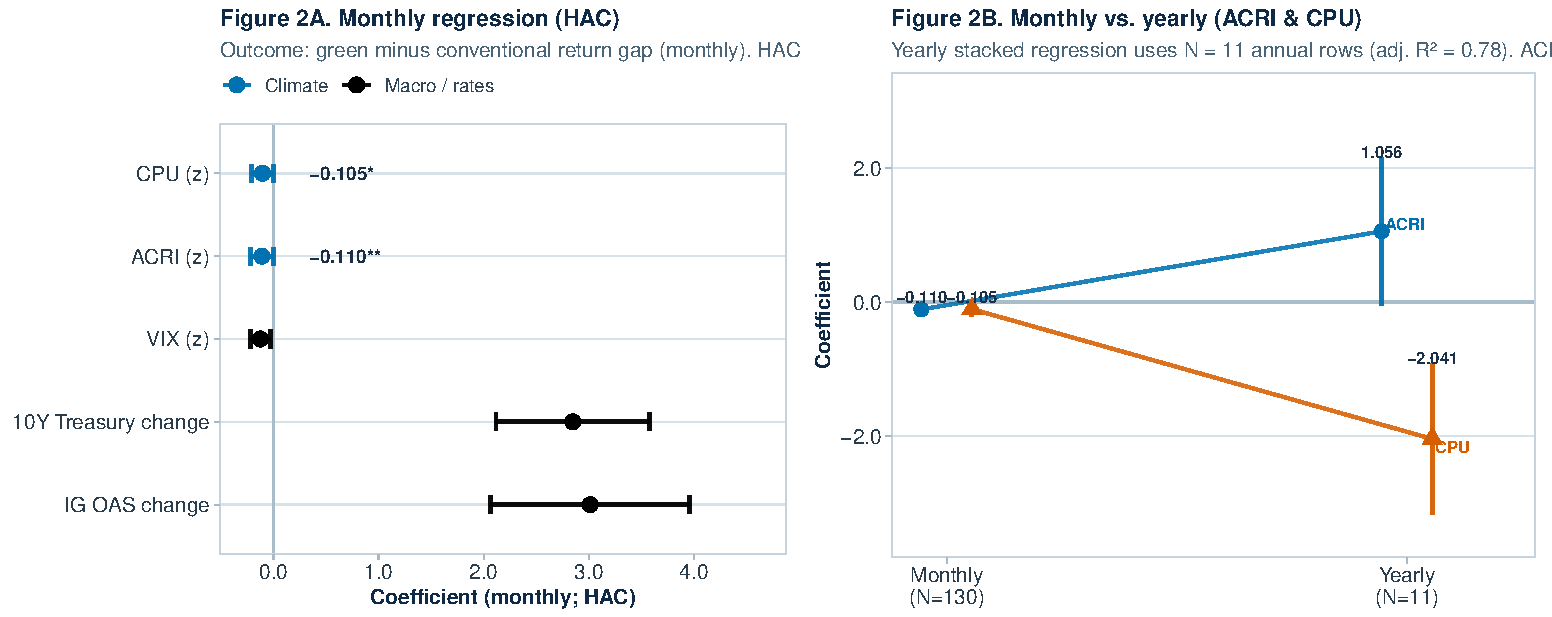
\includegraphics[width=0.88\linewidth]{Final_Paper_Submission_Final_files/figure-latex/climate-evidence-panels-1}}
\caption{Monthly and annual climate-risk coefficients. Panel A reports
monthly coefficient estimates with 95\% HAC confidence intervals on the
green-minus-conventional return differential. Panel B compares ACRI and
CPU on the same standardized z-score scale across horizons with axis labels \textbf{Monthly (N\,=\,130)} versus \textbf{Yearly (N\,=\,11)}. Yearly estimates use OLS intervals from Appendix Table~\ref{tab:app-yearly-frequency}.}
\label{fig:climate-evidence-panels}
\end{figure}

\textbf{Coefficient interpretation for physical risk.}

Higher ACRI months in Table~\ref{tab:monthly-main} line up with green legs lagging their conventional twins after peeling out Treasury yields, IG OAS, and VIX---roughly what we expect when index constituents lean on utilities or project-heavy credit tied to catastrophe headlines (Hypothesis~H4b). Those months also correlate with broader risk-off tone, so the slope mixes hurricane-related stress with garden-variety credit fear. Readers should avoid treating it as a pure hedge story. Section~\ref{bond-level-mechanism-evidence} shows nonprofits that muddy the pooled picture yet vanish inside diversified averages. Appendix lags over one to three months stay insignificant ($p = 0.150$, $0.571$, $0.865$), hinting repricing concentrates in the current month rather than dribbling slowly through reporting delays.

\textbf{Yearly aggregation as a low-power check.}

Stacking eleven fiscal-calendar rows (Appendix Table~\ref{tab:app-yearly-frequency}, $N = 11$) makes Climate Policy Uncertainty pop relative to ACRI in Panel~B of Figure~\ref{fig:climate-evidence-panels}. Nominal \(p\)-values shrink, yet only eleven overlaps remain so standard ``large-sample'' significance stories do not deserve much trust anyway---daggers merely flag direction plus ballpark magnitude. Governments budget yearly while disaster tallies often hit quarterly, which may explain why CPU only catches the light after annual aggregation even though that choice sacrifices statistical power.

\subsection{State dependence}\label{state-dependence}

\begin{table}[!h]
\centering
\caption{\label{tab:krbn-main}Daily regressions of the green-minus-conventional differential on KRBN ETF returns with regime interactions. Three nested specifications: baseline, with rate-hike interactions, and with post-IRA and rate-hike interactions (specifications also include ancillary high-VIX indicators in the full specification as in the estimation code). Huber--White robust standard errors. Sample: August 2020--December 2024 ($N = 1{,}614$ trading days). KRBN lists July 2020 and first non-missing returns align with August in this export.}
\centering
\resizebox{\ifdim\width>\linewidth\linewidth\else\width\fi}{!}{
\fontsize{8}{10}\selectfont
\begin{threeparttable}
\begin{tabular}[t]{lrrrrl}
\toprule
Regressor & Coefficient & Std. error (robust) & $t$ & $p$-value & Sig.\\
\midrule
\addlinespace[0.3em]
\multicolumn{6}{l}{\textbf{Baseline specification}}\\
\hspace{1em}Equity volatility, VIX (z-score) & 0.0138 & 0.0068 & 2.029 & 0.0424 & **\\
\hspace{1em}Change in 10-year Treasury yield & 2.8172 & 0.1169 & 24.104 & 0.0000 & ***\\
\hspace{1em}KRBN carbon-transition ETF return & $-0.0195$ & 0.0039 & $-4.975$ & 0.0000 & ***\\
\addlinespace[0.3em]
\multicolumn{6}{l}{\textbf{With rate-hike interactions}}\\
\hspace{1em}KRBN return $\times$ rate-hike regime & $-0.0156$ & 0.0079 & $-1.960$ & 0.0499 & **\\
\hspace{1em}Equity volatility, VIX (z-score) & 0.0150 & 0.0069 & 2.187 & 0.0288 & **\\
\hspace{1em}Change in 10-year Treasury yield & 2.8182 & 0.1170 & 24.091 & 0.0000 & ***\\
\hspace{1em}KRBN carbon-transition ETF return & $-0.0131$ & 0.0043 & $-3.081$ & 0.0021 & ***\\
\addlinespace[0.3em]
\multicolumn{6}{l}{\textbf{Full: post-IRA and rate-hike interactions}}\\
\hspace{1em}KRBN return $\times$ post-IRA period & 0.0149 & 0.0076 & 1.964 & 0.0495 & **\\
\hspace{1em}KRBN return $\times$ rate-hike regime & $-0.0177$ & 0.0095 & $-1.852$ & 0.0640 & *\\
\hspace{1em}Equity volatility, VIX (z-score) & 0.0252 & 0.0118 & 2.136 & 0.0326 & **\\
\hspace{1em}Change in 10-year Treasury yield & 2.8397 & 0.1183 & 24.005 & 0.0000 & ***\\
\hspace{1em}KRBN carbon-transition ETF return & $-0.0163$ & 0.0052 & $-3.108$ & 0.0019 & ***\\
\bottomrule
\end{tabular}
\begin{tablenotes}
\item \textit{Notes:} Significance: *** $p<0.01$, ** $p<0.05$, * $p<0.10$. The full specification also includes high-VIX indicators and interactions (mirroring the replication code) but those rows are omitted for readability. Reported standard errors reflect the full design. Coefficients summarize patterns conditional on listed controls rather than proving causal shocks.
\end{tablenotes}
\end{threeparttable}}
\end{table}

\textbf{Reading the coefficients.}

In Table~\ref{tab:krbn-main}, tightening cycles strengthen the negative correlation between KRBN returns and our green-minus-conventional spread, matching the idea that dearer credit sharpens transition exposures. Between August 2020 and December 2024 the plain KRBN slope stays negative with $p < 0.01$, while the tightening interaction clears 5\% in the middling model yet drifts toward $p = 0.064$ once post-IRA bells and whistles enter. Post-IRA terms register near $p \approx 0.050$, partly unwinding that drag. Figure~\ref{fig:krbn-regime-plot} contrasts baseline hikes vs.\ hike-window combos (sums near $-0.034$ in these units).

\begin{figure}[H]
{\centering 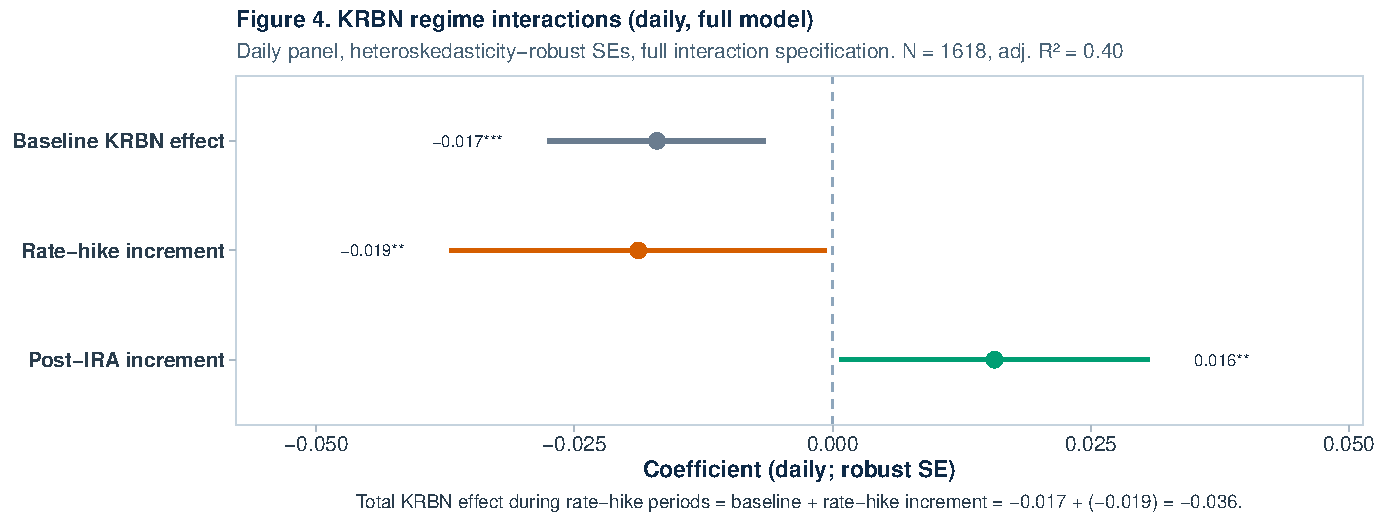
\includegraphics[width=0.88\linewidth]{Final_Paper_Submission_Final_files/figure-latex/krbn-regime-plot-1}}
\caption{KRBN regime decomposition corresponding to Table~\ref{tab:krbn-main}, 95\% robust intervals. Footer annotations sum baseline and hike-period interactions for the tightening-window slope (approximately \(-0.034\) in the August 2020--December 2024 estimation window).}
\label{fig:krbn-regime-plot}
\end{figure}

\subsection{Bond-level mechanism evidence}\label{bond-level-mechanism-evidence}

Alongside indexes we walk through six recognizable U.S.\ issuers. Each month contrasts green-inclusive returns with LQD IG corporates rather than painstakingly rebuilding matched TRACE spreads, while keeping portfolio intuition intact. Appendix Table~\ref{tab:uop-nlp} lists text-based specificity guesses. Figure~\ref{fig:mechanism-profile-plot} aligns those guesses with wedge sizes. Appendix Table~\ref{tab:app-bond-utility-cpu} adds utilities $\times$ CPU dummies and Appendix Table~\ref{tab:app-did-6bond} contrasts early versus late Bloomberg months. Figure~\ref{fig:post-issuance-drift-plot} gives simple averages around month six splits. Tossing Treasury, IG OAS, and VIX into that split leaves a chunky post-gap near $-44$ monthly basis points ($p < 0.001$, Appendix Table~\ref{tab:app-did-6bond}). Patterns echo \citeproc{ref-flammer2021}{Flammer (2021)}: crisp earmarking wording can certify intent without gifting easy outperformance. Nature Conservancy marries sky-high specificity with still-negative bumps, highlighting that prose precision is not alpha by itself, while utilities tilt toward Hypothesis H4's stress branch more than blanket hedges.

\subsection{Daily null results}\label{daily-null-results}

Blaring climate headlines seldom survive side-by-side tests with Treasury swings and IG OAS on Bloomberg's daily tape: overlapping event windows plus trading noise push textbook cutoffs ($p$-values near 5\%/1\%) out of reach regardless of clustering tweaks. Appendix vector autoregressions pairing Treasury impulses, IG spread shocks, and VIX still show Treasury and credit news dominating day-to-day wiggles. Climate-related shocks stay in the passenger seat there. Humans managing cash bonds also rebalance sluggishly versus equity screens, so durable wedges emerge more cleanly in calendar-month totals than hourly headlines. Appendix~\ref{sec:app-var} supports the backbone monthly ACRI story without rewriting it.

\section{Discussion and Limitations}\label{discussion-and-limitations}

Forcing monthly ACRI gradients, eleven-row fiscal aggregates, KRBN-day sensitivities, and six named bonds into one kitchen-sink regression would mash timelines that plainly belong in separate tables anyway. Dedicated monthly, annual, daily, and case-study blocks keep those clocks tidy.

A small unconditional wedge does not mean investors shrug at climate fundamentals. Thick macro controls plus coarse calendar cuts can disguise regime shifts until regressions explicitly allow KRBN/IRA/tightening layers (\citeproc{ref-pham2022}{Pham and Nguyen 2022}; \citeproc{ref-baker2022}{Baker et al. 2022}). Headline calendars alone likewise miss reallocations pinned to calendar month closes (\citeproc{ref-liaw2020}{Liaw 2020}). Slopes summarize patterns, not causal effects from cleanly assigned shocks. Missing macro jitter can still scramble daily residuals. Our LQD comparison is pragmatic, not issuer-by-issuer matched TRACE. Climate Policy Uncertainty at eleven overlapping years paints a blurry picture readers should weigh lightly. Extensions need clearer shock designs, fuller bond panels, tighter emissions bookkeeping, plus investor-flow data—not just sharper wording. We flag those truths beside the pooled monthly standout result.

\section{Conclusion}\label{conclusion}

Green bond spreads respond to overlapping forces simultaneously: Fed cycles that tug duration bets, budgeting calendars where Climate Policy Uncertainty spikes once per fiscal year, carbon-ETF co-movements that stiffen amid tightening regimes, IRA headlines, plus issuer disclosure plays highlighted by six NLP vignettes. Jamming everything into one static intercept hides more than it reveals.

Two patterns survive our replication recipe. Monthly pooled stacks link ACRI negatives to green-vs.-regular gaps once Treasury, IG, and volatility controls imitate how trading desks summarize risk registers ($p \approx 0.048$, Section~\ref{results}). Daily KRBN lines show negative ties to the wedge and extra bite while the Fed hikes, summarized in Table~\ref{tab:krbn-main} for August~2020--December~2024 once screens clear missing dates (KRBN IPO July~2020). Eleven overlapping fiscal aggregates and appendix bond anecdotes help readers interpret timing but merit less argumentative weight simply because \(N\) is tiny.

Trading-day noise still washes mostly through borrowing costs, IG spreads, and VIX moods. Climate series ride those highways as optional passengers, not substitutes for fundamentals investors already watch. Credibly claiming causal arrows would ultimately require richer TRACE-level matched spreads, easier-to-date disaster shocks, plant-level emission ledgers, and allocation data Bloomberg exports cannot fabricate (\citeproc{ref-flammer2021}{Flammer 2021}; \citeproc{ref-sojoudi2025}{Sojoudi et al. 2025}).
\newpage

\section{Appendix}\label{appendix}

\small

\subsection{Variable definitions}\label{sec:app-variables}

\begin{itemize}
\tightlist
\item \textbf{$\Delta r_t$:} Green-minus-conventional return
differential at each frequency (monthly, yearly, daily).
\item \textbf{ACRI:} Actuaries Climate Risk Index, physical climate
risk (\citeproc{ref-acri2020}{American Academy of Actuaries 2020}).
Standardized as \textbf{ACRI\_z}.
\item \textbf{CPU:} Climate Policy Uncertainty index
(\citeproc{ref-gavriilidis2021}{Gavriilidis 2021}, working paper).
Standardized as \textbf{CPU\_z}.
\item \textbf{KRBN:} KraneShares Global Carbon ETF (\texttt{KRBN}) percentage return, our stand-in for carbon-price shocks. Trading begins July~2020, so daily models begin once prices are continuous (here August~2020--December~2024 alongside other Bloomberg extracts).
\item \textbf{LQD:} iShares iBoxx \$ Investment Grade Corporate Bond
ETF total return; bond-level conventional benchmark.
\item \textbf{$\Delta Y^{10y}$:} Monthly, yearly, or daily change in the 10-year Treasury yield matched to whichever regression horizon is running.
\item \textbf{$\Delta \mathrm{OAS}^{IG}$:} First difference of IG
corporate option-adjusted spread.
\item \textbf{VIX / VIX\_z:} CBOE Volatility Index, standardized where used.
\item \textbf{IRA / post-IRA:} Inflation Reduction Act calendar
indicator (after Aug.~16, 2022).
\item \textbf{HAC / robust SE:} Newey--West (monthly time series) and
Huber--White (daily) standard errors.
\item \textbf{UoP:} Use of proceeds (bond prospectus language).
\end{itemize}

\subsection{Yearly horizon check}\label{sec:app-yearly}

\begin{table}[!h]
\centering
\caption{\label{tab:app-yearly-frequency}Yearly climate regression (small-sample caution): dependent variable mirrors the monthly model but summed to yearly rows. OLS standard errors. $N = 11$. Daggers denote nominal $p$-values only---read them as illustrative, not airtight tests.}
\centering
\resizebox{\ifdim\width>\linewidth\linewidth\else\width\fi}{!}{
\fontsize{8}{10}\selectfont
\begin{threeparttable}
\begin{tabular}[t]{lrrrrl}
\toprule
Regressor & Coefficient & Std. error (OLS) & $t$ & Nominal $p$-value & Flag\\
\midrule
Intercept & 0.3326 & 0.5367 & 0.620 & 0.5355 & \\
Climate policy uncertainty (z-score) & $-2.0410$ & 0.5724 & $-3.566$ & 0.0004 & $\dagger\dagger$\\
Physical climate risk (z-score) & 1.0555 & 0.5636 & 1.873 & 0.0611 & $\dagger$\\
KRBN carbon-transition ETF return & $-0.0250$ & 0.0082 & $-3.053$ & 0.0023 & $\dagger\dagger$\\
Change in 10-year Treasury yield & 2.5729 & 0.3447 & 7.464 & 0.0000 & $\dagger\dagger$\\
Equity volatility, VIX (z-score) & 0.2225 & 0.4428 & 0.502 & 0.6153 & \\
\bottomrule
\end{tabular}
\begin{tablenotes}
\item \textit{Notes:} $\dagger\dagger$ flags nominal $p < 0.05$ and $\dagger$ flags nominal $p < 0.10$. With only \(N = 11\) rows, classical ``large sample'' \(p\)-tests are brittle, so treat daggers like traffic lights on sign and size rather than courtroom proof.
\end{tablenotes}
\end{threeparttable}}
\end{table}

\subsection{Six-bond Bloomberg case study (descriptive)}\label{sec:app-bonds}

The six-bond Bloomberg case study is intentionally narrow: it documents how tightly written use-of-proceeds language lines up with benchmark-relative total returns in a slice of recognizable names, not how the entire U.S.\ green corporate market prices climate risk. Technology (Apple), global systemically important banks (JPMorgan Chase, Bank of America), regulated utilities (Duke Energy, NY Electric \& Gas), and a conservation nonprofit (Nature Conservancy) provide variation in both sectoral cash-flow exposure and disclosure posture; price histories run from mid-2023 through year-end 2025. Use-of-proceeds language is parsed with keyword tagging, sentence-transformer embeddings, and a bounded specificity score built from forty-two environmental phrases, echoing the signaling lens in \citeproc{ref-flammer2021}{Flammer (2021)}. Higher scores indicate more concrete, verifiable earmarks rather than generic ``green'' boilerplate.

\begin{table}[!h]
\centering
\caption{\label{tab:uop-nlp}Text-based classification of use of proceeds (UoP), green specificity, and annualized green-bond return relative to the LQD benchmark (same window as the case-study price panel). Specificity is unitless (0--1 range in this sample). $N = 6$ bonds.}
\centering
\resizebox{\ifdim\width>\linewidth\linewidth\else\width\fi}{!}{
\fontsize{8}{10}\selectfont
\begin{threeparttable}
\begin{tabular}[t]{>{\raggedright\arraybackslash}p{1.35in}>{\raggedright\arraybackslash}p{0.95in}>{\raggedright\arraybackslash}p{1.35in}>{\raggedleft\arraybackslash}p{0.82in}>{\raggedleft\arraybackslash}p{0.82in}>{\raggedleft\arraybackslash}p{0.82in}}
\toprule
Issuer & Sector & Use of proceeds & Keyword density & Specificity score & Ann. return diff. vs. LQD (pct.)\\
\midrule
Bank of America & Financials & buildings & 0.189 & 0.657 & $-3.50$\\
JPMorgan Chase & Financials & renewables & 0.106 & 0.523 & $-4.14$\\
Nature Conservancy & Non-Profit & adaptation & 0.304 & 0.945 & $-4.01$\\
Apple Inc. & Technology & renewables & 0.128 & 0.491 & $-4.34$\\
Duke Energy & Utilities & renewables & 0.217 & 0.690 & $-3.98$\\
NY Electric \& Gas & Utilities & renewables & 0.302 & 0.943 & $-7.06$\\
\bottomrule
\end{tabular}
\begin{tablenotes}
\item \textit{Notes:} Descriptive table; significance stars omitted. Annualized return differential is the green-bond total return minus the LQD ETF total return on the overlapping daily window (a return differential, not an option-adjusted spread).
\end{tablenotes}
\end{threeparttable}}
\end{table}

\begin{table}[!h]
\centering
\caption{\label{tab:bond-six-summary}Six-bond case study: monthly return and risk summary over each bond's available Bloomberg history (through 2025-12-31). Annualized return and SD from monthly log returns (pct.); Sharpe is monthly mean over SD (not risk-free adjusted). Correlations use monthly returns vs.\ LQD and vs.\ the BGRN green-bond ETF.}
\centering
\resizebox{\ifdim\width>\linewidth\linewidth\else\width\fi}{!}{
\fontsize{8}{10}\selectfont
\begin{threeparttable}
\begin{tabular}[t]{>{\raggedright\arraybackslash}p{1.30in}>{\raggedright\arraybackslash}p{0.88in}>{\raggedleft\arraybackslash}p{0.60in}>{\raggedleft\arraybackslash}p{0.60in}>{\raggedleft\arraybackslash}p{0.60in}>{\raggedleft\arraybackslash}p{0.60in}>{\raggedleft\arraybackslash}p{0.60in}>{\raggedleft\arraybackslash}p{0.60in}>{\raggedright\arraybackslash}p{1.05in}}
\toprule
Issuer & Sector & N (months) & Ann. return (pct.) & Ann. SD (pct.) & Sharpe & Corr. LQD & Corr. BGRN & Price range\\
\midrule
Bank of America & Financials & 30 & 1.71 & 2.71 & $-0.05$ & 0.78 & 0.77 & 98.94 to 104.73\\
JPMorgan Chase & Financials & 26 & 0.83 & 2.29 & $-0.44$ & 0.93 & 0.93 & 99.83 to 103.68\\
Nature Conservancy & Non-Profit & 26 & 2.78 & 7.14 & 0.13 & 0.46 & 0.40 & 73.23 to 82.22\\
Apple Inc. & Technology & 25 & 2.50 & 2.58 & 0.25 & 0.91 & 0.91 & 93.42 to 99.18\\
Duke Energy & Utilities & 26 & 3.73 & 3.98 & 0.48 & 0.77 & 0.80 & 92.45 to 100.52\\
NY Electric \& Gas & Utilities & 23 & $-4.96$ & 11.23 & $-0.61$ & 0.73 & 0.72 & 75.54 to 87.36\\
\bottomrule
\end{tabular}
\begin{tablenotes}
\item \textit{Notes:} Price fields are clean levels from the case-study extract. Cross-issuer comparisons treat all six as the mechanism-validation sample, not a matched panel.
\end{tablenotes}
\end{threeparttable}}
\end{table}

\begin{figure}[H]
{\centering 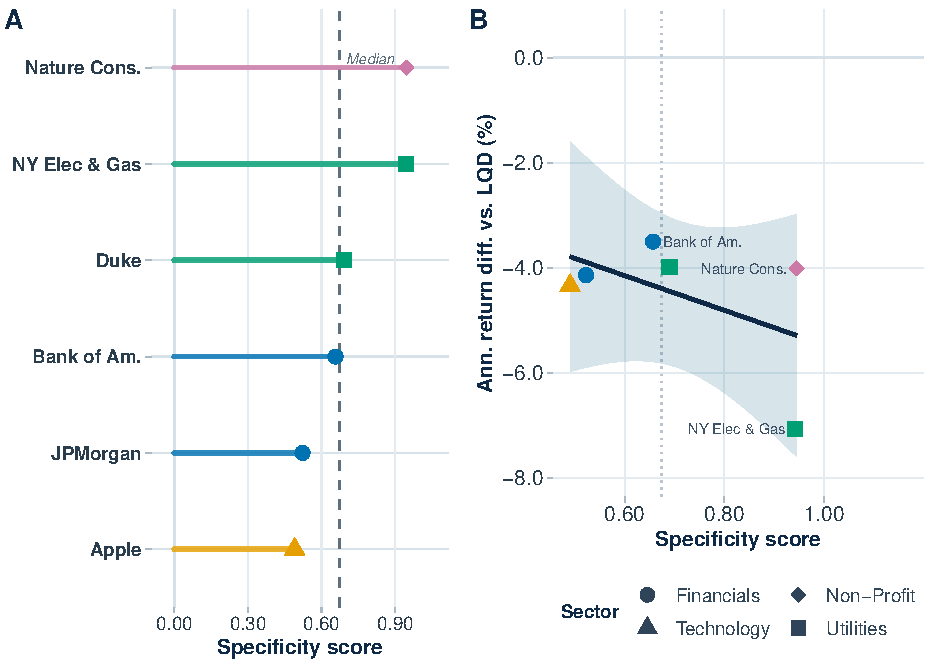
\includegraphics[width=0.90\linewidth]{Final_Paper_Submission_Final_files/figure-latex/mechanism-profile-plot-1}}
\caption{Use-of-proceeds specificity and annualized green-minus-LQD
return differential. Panel A ranks the six issuers by green-specificity
score (dashed line is the sample median). Panel B plots the annualized
green-minus-LQD return differential against specificity (OLS line with
95\% band). Six-bond mechanism sample only.}
\label{fig:mechanism-profile-plot}
\end{figure}

\subsection{Bond-level mechanism regressions}\label{sec:app-bond-mech}

\begin{table}[!h]
\centering
\caption{\label{tab:app-bond-utility-cpu}Bond-month panel (six issuers), climate-policy specification. Dependent variable: green bond monthly return minus conventional IG benchmark monthly return (total-return differential). Huber--White HC1 standard errors. $N = 159$, adjusted $R^2 = 0.640$.}
\centering
\resizebox{\ifdim\width>\linewidth\linewidth\else\width\fi}{!}{
\fontsize{8}{10}\selectfont
\begin{threeparttable}
\begin{tabular}[t]{lrrrr}
\toprule
Regressor & Coef. & Robust SE & $t$ & $p$\\
\midrule
Change in 10-year Treasury yield & 4.0454 & 0.2316 & 17.464 & 0.0000\\
VIX (z-score) & $-0.1117$ & 0.1340 & $-0.834$ & 0.4045\\
CPU (z-score) & 0.1620 & 0.0697 & 2.323 & 0.0202\\
Utility-sector dummy & 0.0506 & 0.1673 & 0.302 & 0.7624\\
Utility $\times$ CPU (z-score) & $-0.0094$ & 0.1183 & $-0.079$ & 0.9367\\
\bottomrule
\end{tabular}
\begin{tablenotes}
\item \textit{Notes:} Standard errors are Huber--White HC1. Coefficients are interpreted as conditional associations, not causal effects. Utility-sector dummy equals one for the two utility names in the six-bond case study.
\end{tablenotes}
\end{threeparttable}}
\end{table}

\begin{table}[!h]
\centering
\caption{\label{tab:app-did-6bond}Bond-level early- vs.\ later-window difference-in-differences on the first-observed-price clock (six issuers). Dependent variable: green bond return minus LQD, monthly. Robust standard errors. $N = 162$, adjusted $R^2 = 0.875$.}
\centering
\resizebox{\ifdim\width>\linewidth\linewidth\else\width\fi}{!}{
\fontsize{8}{10}\selectfont
\begin{threeparttable}
\begin{tabular}[t]{lrrrr}
\toprule
Variable & Coef. & Robust SE & $t$ & $p$\\
\midrule
Intercept & $-0.011$ & 0.073 & $-0.148$ & 0.8824\\
Months 7+ after first observed price month (vs.\ months 1--6) & $-0.444$ & 0.106 & $-4.175$ & 0.0000\\
Change in 10-year Treasury yield & 7.371 & 0.230 & 32.055 & 0.0000\\
Change in IG corporate option-adjusted spread & 11.072 & 0.914 & 12.114 & 0.0000\\
Equity volatility, VIX (z-score) & $-0.172$ & 0.096 & $-1.794$ & 0.0729\\
\bottomrule
\end{tabular}
\begin{tablenotes}
\item \textit{Notes:} The post indicator compares months 7--18 to months 1--6 on a clock anchored at the first non-missing Bloomberg price for each bond, not at issuance. With only six underlying bond units, \(p\)-values primarily indicate direction and within-sample precision rather than population-level inference, even though the regression contains monthly observations.
\end{tablenotes}
\end{threeparttable}}
\end{table}

\begin{figure}[H]
{\centering 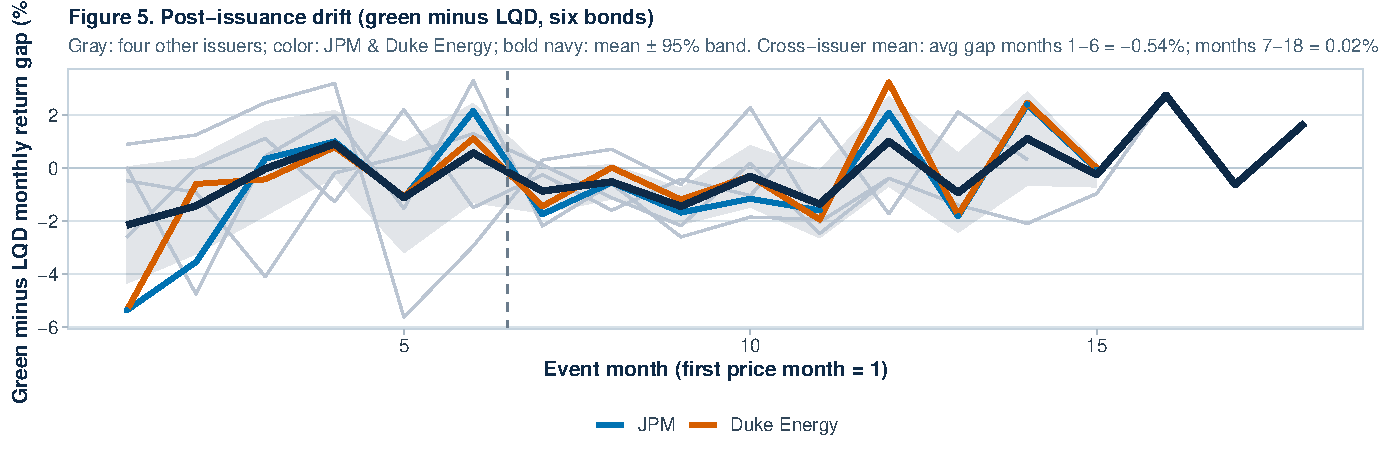
\includegraphics[width=0.88\linewidth]{Final_Paper_Submission_Final_files/figure-latex/post-issuance-drift-plot-1}}
\caption{Six-bond green-minus-LQD monthly gaps by Bloomberg price-calendar month index. Thin gray issuer lines stay in the plot for transparency. JPMorgan Chase and Duke Energy stay saturated for readability. The thick navy curve with ribbon is the cross-issuer mean and 95\% interval. Horizontal dashes bracket mean gaps before versus after month six. The vertical dashed line splits the DiD windows in Table~\ref{tab:app-did-6bond}. Month 1 is each bond's first observed Bloomberg price.}
\label{fig:post-issuance-drift-plot}
\end{figure}

\subsection{Daily VAR diagnostics}\label{sec:app-var}

Appendix vector autoregression charts map one-day responses to Treasury, IG spread, volatility, and climate surprises. System~3 stacks the green-minus-conventional spread beside climate series. System~4 repeats the exercise after stripping interest-rate exposure from the spread. The takeaway is routine: Treasury shocks, IG shocks, and VIX still chew through most next-day forecast swings, while climate-only surprises claim a modest slice.

\begin{figure}[H]
{\centering 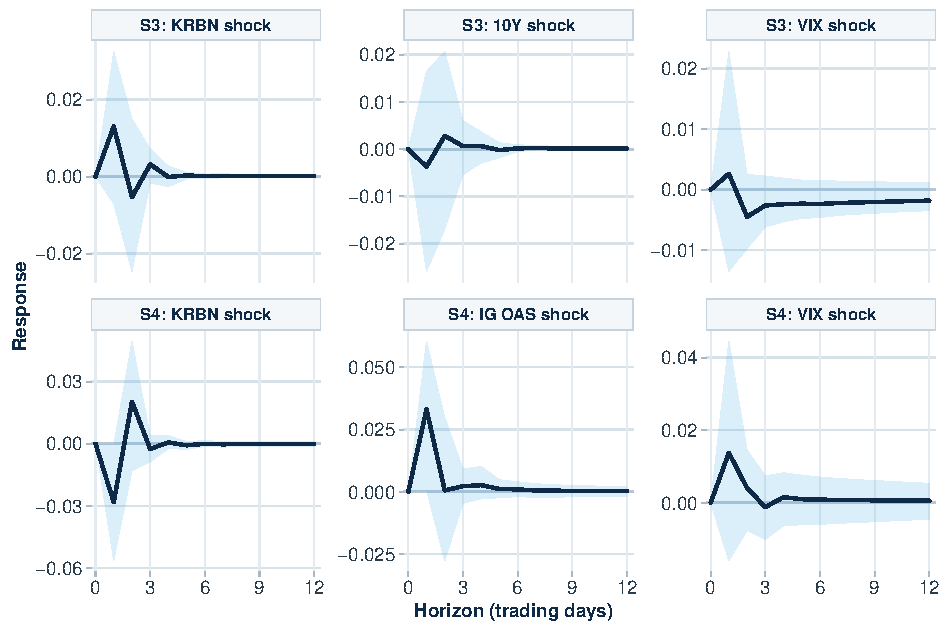
\includegraphics[width=0.88\linewidth]{Final_Paper_Submission_Final_files/figure-latex/var-irf-compact-1}}
\caption{Daily VAR impulse response functions (IRFs). Each small panel
shows the response of the target series to one structural shock over
trading days. Lines show point IRFs. Ribbons are bootstrap 95\% bands.
S3 = green--conventional differential system. S4 = rate-hedged
differential.}
\label{fig:var-irf-compact}
\end{figure}

\begin{figure}[H]
{\centering 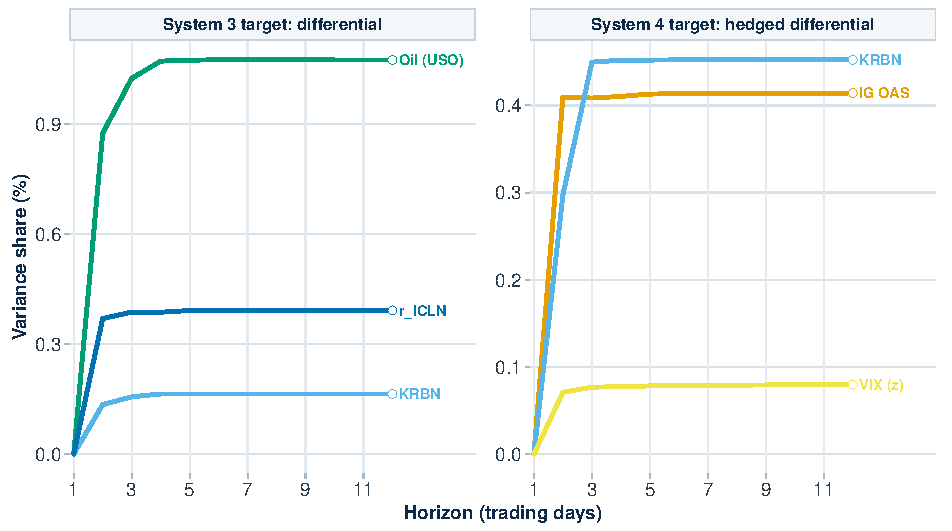
\includegraphics[width=0.88\linewidth]{Final_Paper_Submission_Final_files/figure-latex/var-fevd-compact-1}}
\caption{Daily VAR forecast error variance decompositions (FEVDs).
Each colored line is the share of forecast-error variance attributable
to one shock at the indicated horizon (days). Left vs.\ right panel:
differential vs.\ rate-hedged differential target.}
\label{fig:var-fevd-compact}
\end{figure}

\clearpage

\section*{References}\label{references}
\addcontentsline{toc}{section}{References}

\protect\phantomsection\label{refs}
\begin{CSLReferences}{1}{1}
\bibitem[\citeproctext]{ref-acri2020}
American Academy of Actuaries. 2020. {``Actuaries Climate Risk Index:
Preliminary Findings.''} Policy \& Research Report. Washington, DC.
\url{https://actuary.org/resources/actuaries-climate-risk-index-preliminary-findings/}

\bibitem[\citeproctext]{ref-agliardi2021}
Agliardi, Rosella, and Emanuele Agliardi. 2021. {``Pricing
Climate-Related Risks in the Bond Market.''} \emph{Journal of Financial
Stability} 53: 100815.

\bibitem[\citeproctext]{ref-baker2022}
Baker, Malcolm, Daniel Bergstresser, George Serafeim, and Jeffrey
Wurgler. 2022. {``The Pricing and Ownership of U.S. Green Bonds.''}
\emph{Annual Review of Financial Economics} 14: 415--37.

\bibitem[\citeproctext]{ref-bolton2023}
Bolton, Patrick, and Marcin Kacperczyk. 2023. {``Global Pricing of
Carbon-Transition Risk.''} \emph{Journal of Finance} 78 (4): 3677--723.

\bibitem[\citeproctext]{ref-flammer2021}
Flammer, Caroline. 2021. {``Corporate Green Bonds.''} \emph{Journal of
Financial Economics} 142 (2): 499--516.

\bibitem[\citeproctext]{ref-gavriilidis2021}
Gavriilidis, Konstantinos. 2021. {``Measuring Climate Policy
Uncertainty.''} \emph{SSRN Electronic Journal} (working paper, not formally peer-reviewed), https://doi.org/10.2139/ssrn.3847388.

\bibitem[\citeproctext]{ref-karpf2018}
Karpf, Aaron, and Antoine Mandel. 2018. {``The Changing Value of the
"Green" Label on the U.S. Municipal Bond Market.''} \emph{Nature Climate
Change} 8 (2): 161--65.

\bibitem[\citeproctext]{ref-li2024}
Li, Wenqi, Suhas Saigal, and Peter Adriaens. 2024. {``Impact of Flooding
and Drought Risks on the Cost of Bond Financing for Water Utilities.''}
\emph{Environmental Science \& Technology} 58 (32): 14068--79.

\bibitem[\citeproctext]{ref-liaw2020}
Liaw, Kwang Teck. 2020. {``Survey of Green Bond Pricing and Investment
Performance.''} \emph{Journal of Risk and Financial Management} 13 (9):
182.

\bibitem[\citeproctext]{ref-macaskill2021}
MacAskill, Stephen, Eduardo Roca, Binh Liu, Rodney A. Stewart, and Oz
Sahin. 2021. {``Is There a Green Premium in the Green Bond Market? A
Systematic Review Revealing Premium Determinants.''} \emph{Journal of
Cleaner Production} 280: 124491.

\bibitem[\citeproctext]{ref-mari2024}
Mar'i, M. 2024. {``The Impact of Financial Stress and Uncertainty on
Green and Conventional Bonds and Stocks: A Nonlinear and Nonparametric
Quantile Analysis.''} \emph{Risks} 12 (8): 120.

\bibitem[\citeproctext]{ref-painter2020}
Painter, Marcus. 2020. {``An Inconvenient Cost: The Effects of Climate
Change on Municipal Bonds.''} \emph{Journal of Financial Economics} 135
(2): 468--82.

\bibitem[\citeproctext]{ref-park2020}
Park, Daejin, Jimin Park, and Doojin Ryu. 2020. {``Volatility Spillovers
Between Equity and Green Bond Markets.''} \emph{Sustainability} 12 (9):
3722.

\bibitem[\citeproctext]{ref-partridge2020}
Partridge, Candice, and Francesca Medda. 2020. {``The Evolution of
Pricing Performance of Green Municipal Bonds.''} \emph{Journal of
Sustainable Finance \& Investment} 10 (2): 133--54.

\bibitem[\citeproctext]{ref-pham2022}
Pham, Linh, and Cuong Phu Nguyen. 2022. {``How Do Stock, Oil, and
Economic Policy Uncertainty Influence the Green Bond Market?''}
\emph{Finance Research Letters} 45: 102128.

\bibitem[\citeproctext]{ref-seltzer2022}
{Seltzer, Luke, Shirley Sun, et al.} 2022. \emph{Climate Regulatory
Risks and Corporate Bonds}. Federal Reserve Bank of New York Staff
Report 1011.

\bibitem[\citeproctext]{ref-smull2023}
Smull, Emily, Daniel Walsh, Colin Sullivan, and Caleb Ponder. 2023.
{``Climate, Race, and the Cost of Capital in the Municipal Bond
Market.''} \emph{PLOS ONE} 18 (8): e0288979.

\bibitem[\citeproctext]{ref-sojoudi2025}
Sojoudi, Mohammad, Carole Bernard, Pierre Dupuy, and Gareth Peters.
2025. {``Green Spread of U.S. Municipal Bonds.''} \emph{Annals of
Operations Research}.

\bibitem[\citeproctext]{ref-tiwari2022}
Tiwari, Aviral Kumar, Emmanuel J. A. Abakah, David Gabauer, and Richmond
A. Dwumfour. 2022. {``Dynamic Spillover Effects Among Green Bond,
Renewable Energy Stocks and Carbon Markets During COVID-19 Pandemic.''}
\emph{Global Finance Journal} 51: 100692.

\end{CSLReferences}

\end{document}
